\documentclass[a4paper,12pt]{article}

\usepackage[utf8]{inputenc}
\usepackage[T1]{fontenc}
\usepackage{amsmath}
\usepackage{booktabs}
\usepackage{graphicx}
\usepackage{geometry}
\geometry{margin=2.5cm}
\usepackage{xcolor}
\usepackage{listings}
\usepackage{hyperref}
\usepackage{float}
\hypersetup{colorlinks=true, linkcolor=blue!50!black, urlcolor=blue!50!black}
\renewcommand{\tablename}{Tabela}
\renewcommand{\figurename}{Figura}
\renewcommand{\lstlistingname}{Código}

% ---------- Configuração do realce de sintaxe (C) ----------
\definecolor{codebg}{RGB}{247,247,247}
\definecolor{codekw}{RGB}{0,0,180}
\definecolor{codecomment}{RGB}{0,128,0}
\definecolor{codestring}{RGB}{163,21,21}
\definecolor{framecolor}{RGB}{200,200,200}

\lstdefinestyle{cstyle}{
    language=C,
    backgroundcolor=\color{codebg},
    basicstyle=\ttfamily\footnotesize,
    keywordstyle=\color{codekw}\bfseries,
    commentstyle=\color{codecomment}\itshape,
    stringstyle=\color{codestring},
    numberstyle=\tiny\color{gray},
    numbers=left,
    numbersep=6pt,
    frame=single,
    rulecolor=\color{framecolor},
    breaklines=true,
    breakatwhitespace=false,
    showstringspaces=false,
    tabsize=4,
    captionpos=b,
    columns=flexible,
    morekeywords={size_t},
    extendedchars=true,
    literate=
        {á}{{\'a}}1 {à}{{\`a}}1 {â}{{\^a}}1 {ã}{{\~a}}1
        {é}{{\'e}}1 {ê}{{\^e}}1 {í}{{\'i}}1
        {ó}{{\'o}}1 {ô}{{\^o}}1 {õ}{{\~o}}1
        {ú}{{\'u}}1 {ü}{{\"u}}1 {ç}{{\c c}}1
        {Á}{{\'A}}1 {À}{{\`A}}1 {Â}{{\^A}}1 {Ã}{{\~A}}1
        {É}{{\'E}}1 {Ê}{{\^E}}1 {Í}{{\'I}}1
        {Ó}{{\'O}}1 {Ô}{{\^O}}1 {Õ}{{\~O}}1
        {Ú}{{\'U}}1 {Ü}{{\"U}}1 {Ç}{{\c C}}1
}

\title{Tarefa 13: Avaliação da Escalabilidade com Afinidade de Threads}
\author{Israel Soares de Castro Filho \\ Matrícula: 20250070780}
\date{}

\begin{document}

\maketitle

\section{Introdução}

A \textbf{afinidade de threads} define em quais CPUs cada thread pode executar. Sem afinidade, o sistema operacional escolhe e pode migrar as threads a qualquer momento; com afinidade, cada thread fica restrita a um \emph{lugar} (\emph{place}), que pode ser uma CPU lógica, um núcleo ou um processador inteiro.

O objetivo desta tarefa é avaliar como as políticas de afinidade do OpenMP, controladas por \texttt{OMP\_PROC\_BIND} e \texttt{OMP\_PLACES}, alteram a escalabilidade forte do código de Navier-Stokes 2D (versão 4 da tarefa 12) em um nó do NPAD.

\section{Metodologia}

\paragraph{Ambiente.} Nó da partição \texttt{amd-512} do NPAD, com 2 processadores AMD EPYC 7713 (128 núcleos físicos no total) e 2 threads por núcleo (SMT), somando 256 CPUs lógicas.

\paragraph{Código.} Versão 4 da tarefa 12, sem alteração no cálculo. A única mudança foi permitir escolher a política de afinidade e registrar em que CPU cada thread executa, para contar migrações. Nos experimentos, a política e os lugares foram definidos pelas variáveis de ambiente.

\paragraph{Experimento.} Malha $2048\times2048$, 210 passos de tempo, de 1 a 256 threads (potências de 2) e 5 repetições de cada caso. O \emph{speedup} é calculado em relação à execução sem afinidade com 1 thread (2,667 s). As afinidades avaliadas estão na Tabela~\ref{tab:afin}.

\begin{table}[ht]
\centering
\small
\begin{tabular}{@{}p{3.1cm}p{12.4cm}@{}}
\toprule
\texttt{OMP\_PROC\_BIND} & O que faz \\
\midrule
\texttt{false} & Sem afinidade: o sistema operacional pode migrar as threads entre CPUs. \\
\texttt{true} & Cada thread fica fixa no lugar onde foi criada, seguindo a ordem dos lugares. \\
\texttt{close} & Threads em lugares consecutivos, o mais perto possível da thread mestre (compacto). \\
\texttt{spread} & Threads distribuídas por igual entre todos os lugares (espalhado pelo nó). \\
\texttt{master} & Todas as threads no mesmo lugar da thread mestre. \\
\midrule
\texttt{OMP\_PLACES} & Lugar \\
\midrule
\texttt{threads} & Uma CPU lógica (uma thread de hardware). \\
\texttt{cores} & Um núcleo físico, com suas 2 threads SMT. \\
\texttt{sockets} & Um processador inteiro (64 núcleos); a thread ainda pode se mover dentro dele. \\
\bottomrule
\end{tabular}
\caption{Políticas de afinidade e tipos de lugar avaliados.}
\label{tab:afin}
\end{table}

Foram testadas 9 combinações: \texttt{false}; \texttt{true} com \texttt{cores}; \texttt{close} e \texttt{spread} com \texttt{threads}, \texttt{cores} e \texttt{sockets}; e \texttt{master} com \texttt{cores}. Os scripts e o código completo estão no Apêndice.

\section{Resultados}

A Tabela~\ref{tab:speedup} mostra o speedup médio de cada combinação e a Figura~\ref{fig:speedup} mostra as mesmas curvas. Em todas as execuções o erro máximo em relação à solução analítica foi o mesmo ($1{,}1\times10^{-7}$), ou seja, a afinidade muda apenas o tempo, não o resultado.

\begin{table}[H]
\centering
\small
\setlength{\tabcolsep}{4.5pt}
\begin{tabular}{lrrrrrrrrr}
\toprule
Política \textbar\ lugares & 1 & 2 & 4 & 8 & 16 & 32 & 64 & 128 & 256 \\
\midrule
\texttt{false} & 1,0 & 1,9 & 3,8 & 7,5 & 14,1 & 27,5 & 32,5 & 14,6 & 15,4 \\
\texttt{true \textbar cores} & 1,1 & 2,0 & 2,8 & 2,9 & 4,3 & 28,1 & 43,8 & 76,8 & 78,3 \\
\texttt{close \textbar threads} & 0,97 & 0,99 & 1,9 & 2,7 & 2,9 & 4,3 & 25,7 & 39,3 & 71,0 \\
\texttt{close \textbar cores} & 1,0 & 2,0 & 2,8 & 2,9 & 4,3 & 28,9 & 44,6 & 76,2 & 77,9 \\
\texttt{close \textbar sockets} & 0,99 & 1,8 & 3,7 & 7,0 & 8,2 & 23,5 & 41,6 & 24,2 & 28,7 \\
\texttt{spread \textbar threads} & 0,97 & 1,9 & 3,7 & 7,4 & 14,5 & 28,0 & 51,1 & 75,3 & 77,3 \\
\texttt{spread \textbar cores} & 1,0 & 1,8 & 3,8 & 7,5 & 14,4 & 28,3 & 50,5 & 75,9 & 76,8 \\
\texttt{spread \textbar sockets} & 0,99 & 1,9 & 4,1 & 6,6 & 7,5 & 26,4 & 41,5 & 26,0 & 34,3 \\
\texttt{master \textbar cores} & 1,0 & 1,0 & 0,84 & 0,55 & 0,45 & 0,21 & 0,10 & 0,05 & 0,02 \\
\bottomrule
\end{tabular}

\caption{Speedup médio (5 repetições) por número de threads.}
\label{tab:speedup}
\end{table}

\begin{figure}[H]
\centering
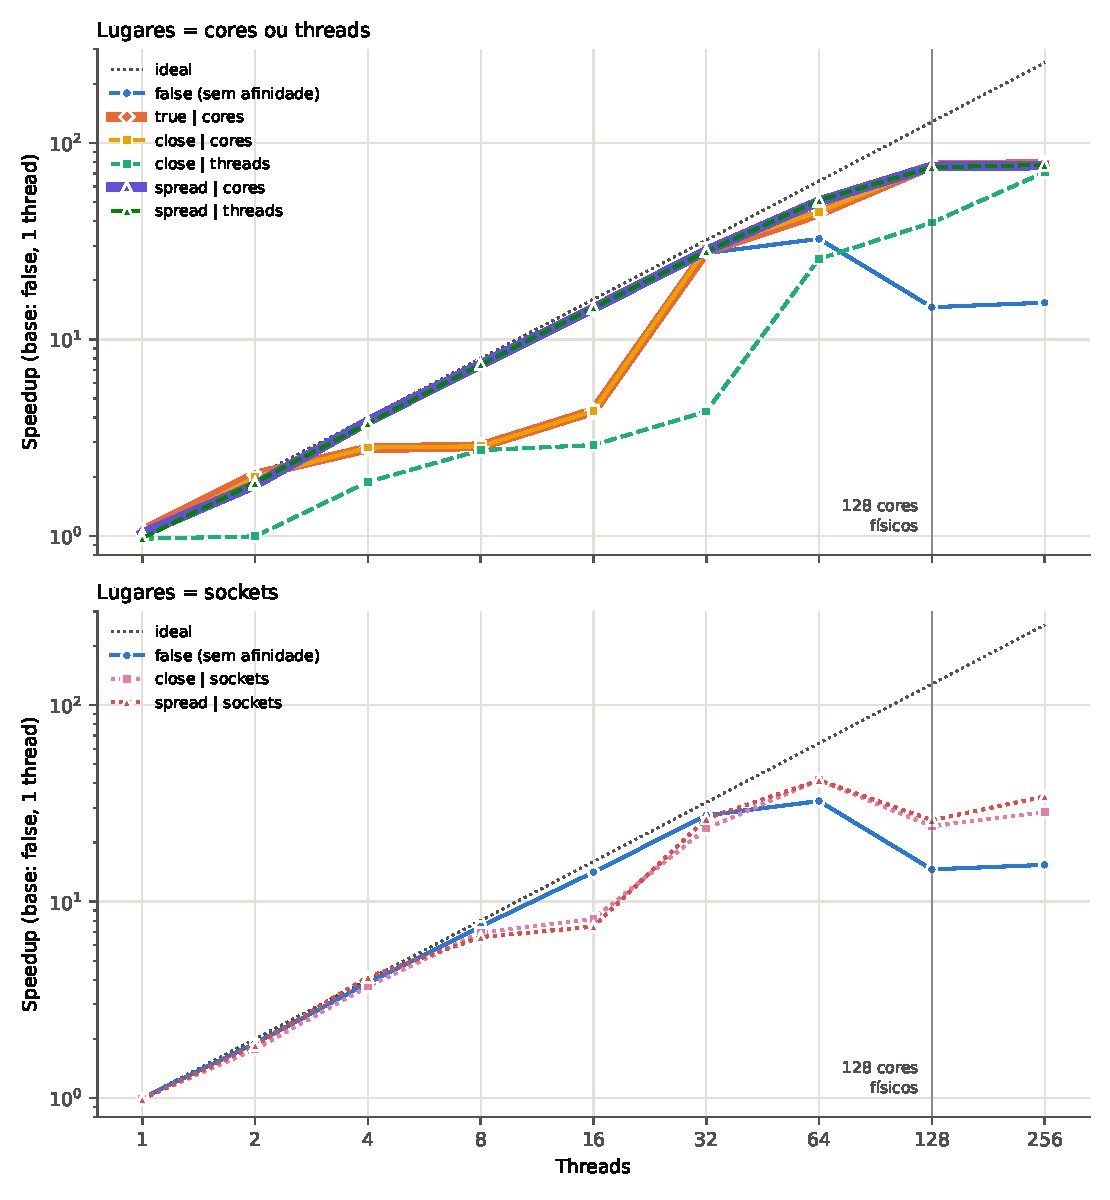
\includegraphics[width=\textwidth]{../fig/fig1_speedup.pdf}
\caption{Speedup em função do número de threads. Acima, lugares \texttt{cores} e \texttt{threads}; abaixo, lugares \texttt{sockets}. As curvas de \texttt{true|cores} e \texttt{close|cores} coincidem, assim como as de \texttt{spread|cores} e \texttt{spread|threads}.}
\label{fig:speedup}
\end{figure}

Com 1 thread todos os casos ficam entre 0,97 e 1,06, o que dá uma ideia do ruído de medição. Nos casos sem fixação por núcleo, os tempos variaram mais entre as repetições.

\section{Análise}

\begin{itemize}
    \item \textbf{Sem afinidade (\texttt{false}).} O sistema operacional escolhe onde cada thread executa. Funciona bem até 32 threads (speedup 27,5), mas com 128 e 256 threads o speedup cai para 14,6 e 15,4 e os tempos ficam instáveis. Sem controle, as threads acabam mal distribuídas entre os núcleos, e a mais lenta atrasa todas.

    \item \textbf{\texttt{spread}.} Espalha as threads por todo o processador e é a política que melhor se mantém próxima do ideal em toda a faixa: speedup de 14,4 com 16 threads, 28,3 com 32 e 50,5 com 64 (contra 32,5 sem afinidade).

    \item \textbf{\texttt{true} e \texttt{close} com \texttt{cores}.} Agrupam as threads nos primeiros núcleos. Com poucas threads isso atrapalha: o speedup fica parado em cerca de 2,8 com 4 e 8 threads e chega a só 4,3 com 16. A partir de 32 threads o desempenho se equipara ao dos demais (28,1 a 28,9). As duas políticas deram o mesmo resultado.

    \item \textbf{Todos os núcleos em uso (128 threads).} Qualquer fixação por núcleo dá praticamente o mesmo resultado (75 a 77). Com 256 threads (2 threads por núcleo, SMT) o ganho é de apenas 2\% (78,3), então usar o SMT não compensa neste código.

    \item \textbf{\texttt{close} com \texttt{threads}.} Pelos resultados, as threads ocupam as duas CPUs lógicas de cada núcleo antes de passar para o próximo, e por isso usam só metade dos núcleos: com 2 threads não há ganho (0,99) e com 16 o speedup é só 2,9. Só se aproxima dos demais com 256 threads (71).

    \item \textbf{Lugares \texttt{sockets}.} A thread fica presa ao processador, mas o sistema ainda escolhe o núcleo. O resultado fica entre o \texttt{false} e a fixação por núcleo: com 128 e 256 threads o speedup é de 24 a 34, melhor que sem afinidade (14,6 e 15,4), mas bem abaixo da fixação por núcleo (76 a 78).

    \item \textbf{\texttt{master}.} Coloca todas as threads no mesmo núcleo. Com 2 threads não há ganho (1,01) e, com mais threads, o programa fica mais lento que o serial: com 256 threads o cálculo leva 109,6 s, cerca de 41 vezes mais que com 1 thread (Figura~\ref{fig:master}).
\end{itemize}

\begin{figure}[H]
\centering
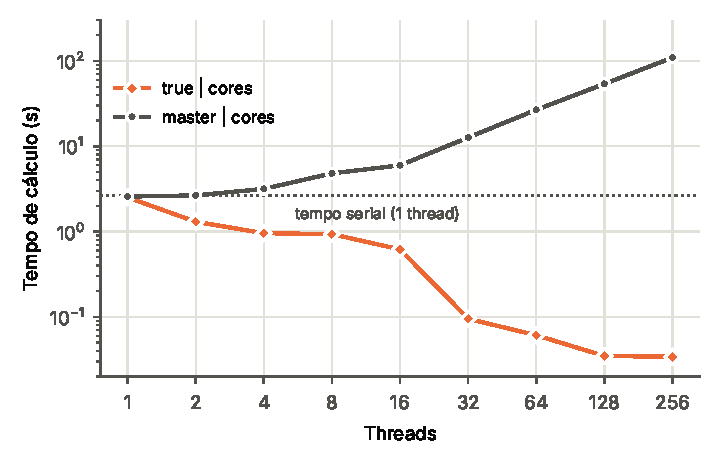
\includegraphics[width=0.62\textwidth]{../fig/fig2_master.pdf}
\caption{Tempo de cálculo de \texttt{master|cores} comparado a \texttt{true|cores}. Com \texttt{master}, mais threads significam mais tempo.}
\label{fig:master}
\end{figure}

\section{Conclusão}

A afinidade não faz diferença com 1 thread, mas importa cada vez mais conforme o número de threads cresce: com 128 threads o speedup é 14,6 sem afinidade e de 75 a 77 fixando cada thread em um núcleo.

\begin{itemize}
    \item Usar \texttt{spread} com lugares \texttt{cores} (ou \texttt{threads}) quando houver menos threads que núcleos: é a política com melhor desempenho em toda a faixa.
    \item Com todos os núcleos em uso, qualquer fixação por núcleo serve (\texttt{true}, \texttt{close} ou \texttt{spread} com \texttt{cores}). Usar o SMT (256 threads) quase não compensa.
    \item Evitar \texttt{false} com muitas threads (acima de 32), lugares \texttt{sockets}, \texttt{close} com \texttt{threads} e \texttt{master}.
\end{itemize}

Os resultados valem para uma única malha ($2048\times2048$).

\newpage
\appendix

\section{Código-Fonte}

\lstinputlisting[style=cstyle, caption={Código \texttt{tarefa13.c}: versão 4 com afinidade de threads.}]{../src/tarefa13.c}

\lstinputlisting[style=cstyle, language=bash, caption={Script \texttt{tarefa13.sh}: execução no NPAD.}]{../src/tarefa13.sh}

\end{document}